\iffalse
\let\negmedspace\undefined
\let\negthickspace\undefined
\documentclass[journal,12pt,twocolumn]{IEEEtran}
\usepackage{cite}
\usepackage{amsmath,amssymb,amsfonts,amsthm}
\usepackage{algorithmic}
\usepackage{graphicx}
\usepackage{textcomp}
\usepackage{xcolor}
\usepackage{txfonts}
\usepackage{listings}
\usepackage{enumitem}
\usepackage{mathtools}
\usepackage{gensymb}
\usepackage{comment}
\usepackage[breaklinks=true]{hyperref}
\usepackage{tkz-euclide} 
\usepackage{listings}
\usepackage{gvv}                                        
%\def\inputGnumericTable{}                                 
\usepackage[latin1]{inputenc}                                
\usepackage{color}                                            
\usepackage{array}                                            
\usepackage{longtable}                                       
\usepackage{calc}                                             
\usepackage{multirow}                                         
\usepackage{hhline}                                           
\usepackage{ifthen}                                           
\usepackage{lscape}
\usepackage{tabularx}
\usepackage{array}
\usepackage{float}


\newtheorem{theorem}{Theorem}[section]
\newtheorem{problem}{Problem}
\newtheorem{proposition}{Proposition}[section]
\newtheorem{lemma}{Lemma}[section]
\newtheorem{corollary}[theorem]{Corollary}
\newtheorem{example}{Example}[section]
\newtheorem{definition}[problem]{Definition}
\newcommand{\BEQA}{\begin{eqnarray}}
\newcommand{\EEQA}{\end{eqnarray}}
\newcommand{\define}{\stackrel{\triangle}{=}}
\theoremstyle{remark}
\newtheorem{rem}{Remark}
\begin{document}

\bibliographystyle{IEEEtran}
\vspace{3cm}

\title{Question 37, EE Gate 2022}
\author{EE23BTECH11017 - Eachempati Mihir Divyansh$^{*}$}
\maketitle
\newpage
\bigskip

\renewcommand{\thefigure}{\theenumi}
\renewcommand{\thetable}{\theenumi}
\textbf{Question:} An LTI system is shown in the figure where $$H\brak{s}= \frac{100}{s^2+0.1s+10}$$ The steady state output of the system for an input $x\brak{t}$ is given by $y\brak{t}=a+b\sin{\brak{10t+\theta}}$. The values of $'a'$ and $'b'$ are \\\\
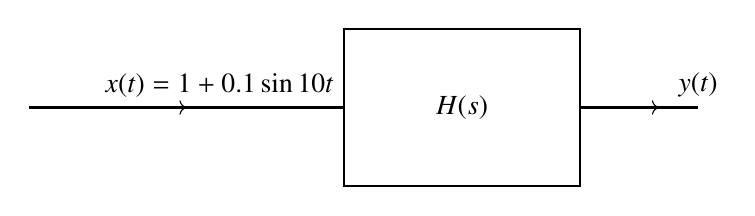
\begin{tikzpicture}
    \draw [thick, draw=black] (-2,-1) -- (2,-1) node[anchor=south east] {$x(t)=1+0.1\sin{\brak{10t}}$};
    \draw [thick,draw=black] (2,0) rectangle (5,-2) ;
    \draw [thick,draw=black] (5,-1) -- (6.5,-1) node[anchor=south] {$y(t)$};
    \draw [->] (-2,-1)--(0,-1);
    \draw [->] (5,-1)--(6,-1);
    \draw (3.5, -1) node[] {$H(s)$};
\end{tikzpicture}

\solution \\
\fi
\begin{table}[h]
    \centering
    \begin{tabular}{|c|c|c|}
    \hline
   Symbol & Value & Description \\
    \hline
    $x\brak{t}$ & $1+0.1\sin{\brak{10t}}$ & Input Signal\\ [2ex]
    \hline
    $y\brak{t}$ & ? & Output of the system\\[2ex]
    \hline 
    $H\brak{s}$ & $\frac{100}{s^2+0.1s+10}$ & Impulse Response\\[2ex]
    \hline
\end{tabular}
    \caption{Given Information} 
    \label{37.Gate22.EE.tab: 1}                                                                                                                                                                                                 
\end{table}
\begin{enumerate}
\item \textbf{Theory: } If a sinusoidal input is given to a system, whose transfer function is known, the output can be calculated as follows
\begin{align}
    y(t)&=h(t)*x(t)\\
    Y(s)&=H(s)X(s)
\end{align}
Let $s=j\omega$
\begin{align}
    Y(j\omega)&=H(j\omega)X(j\omega)
\end{align}
If $\Phi$ is the phase of $H(j\omega)$, 
\begin{align}
    H(j\omega)=\abs{H(j\omega)}e^{j\Phi(\omega)}
\end{align}
If $x(t)=\cos{(\omega_0t)}$, 
\begin{align}
    X(j\omega)&=\pi \brak{\delta(\omega-\omega_0)+\delta(\omega+\omega_0)}
   % \implies X(f)&=\frac{1}{2}\brak{\delta(f-f_0)+\delta(f+f_0)}
\end{align}
Now,
\begin{align}
    Y(j\omega)=&\brak{\delta(\omega-\omega_0)+\delta(\omega+\omega_0)}\abs{H(j\omega)}e^{j\Phi(\omega)}\\
\end{align}
Since $\abs{H(j\omega)}\delta(\omega-\omega_0)$ is zero everywhere except at $\omega_0$ 
\begin{align}
    Y(j\omega)=&\abs{H(j\omega_0)}e^{j\Phi(\omega_0)}\delta(\omega-\omega_0) \\&+ \abs{H(-j\omega_0)}e^{j\Phi(-j\omega_0)}\delta(\omega+\omega_0)
\end{align}
As $h(t)$ is real, $${H(\omega)}={H^{*}(-\omega)}$$ 
 $$\Phi(-\omega_0)=-\Phi(\omega_0)$$
Hence 
 \begin{align}
    Y(\omega)= \abs{H(\omega_0)}\brak{e^{j\Phi(\omega_0)}\delta(\omega-\omega_0) + e^{-j\Phi(\omega_0)}\delta(\omega+\omega_0)}
\end{align}
Taking Inverse Fourier Transform, 
\begin{align}
    &\delta(\omega-\omega_0) \system{F} \frac{1}{2}e^{j\omega_0t}\\
    &\implies y(t)=\abs{H(\omega_0)}\frac{1}{2}\brak{e^{j\brak{\omega_0t+\Phi(\omega_0)}}+e^{-j\brak{\omega_0t+\Phi(\omega_0)}}}\\
    &\implies y(t) = \abs{H(\omega_0)}\cos{\brak{\omega_0t+\Phi(\omega_0)}}
\end{align}
\item The given input can be assumed to be a superposition of $u(t)$ and $0.1\sin{\brak{\omega_0t}}u(t)$. $$\omega_0=0 \text{ and }\omega_0=10$$ for the constant input and the sinusoidal input respectively.
\begin{align}
    y(t)=\abs{H(0)}+\abs{H(10)}\sin{\brak{10t+\Phi(10)}}
\end{align}
Here
\begin{align}
    H(\omega)&=\frac{100}{(j\omega)^2+0.1(j\omega)+10}\\
    \implies H(\omega)&=\frac{100}{10-\omega^2+j(0.1\omega)}\\
    \implies \abs{H(\omega)}&=\frac{100}{\sqrt{(10-\omega^2)^2+(0.1\omega)^2}}\\
    \therefore \abs{H(0)}&=10 \text{ and } \abs{H(10)}\approx 1
\end{align}
The phase $\Phi(\omega)$ is given by 
\begin{align}
    \Phi(\omega)&=\tan^{-1}\frac{0.1\omega}{\omega^2-10}\\
    \implies \Phi(10)&=\tan^{-1} \frac{1}{90}
\end{align}
Hence the output of the system 
\begin{align}
    y(t)=10+\sin{(10t+\tan^{-1} \frac{1}{90})}
\end{align}
Hence $a=10$ and $b=1$ 
\begin{figure}[h]
    \centering
    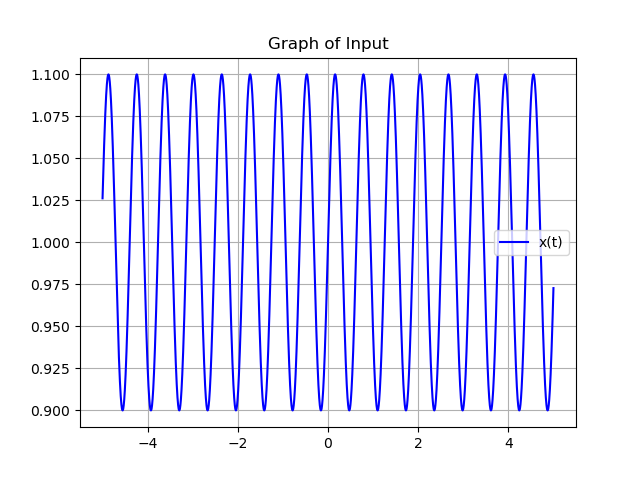
\includegraphics[width=\columnwidth]{2022/EE/37/figs/input.png}
    \caption{Input of the system, $x(t)$} 
\end{figure}
\begin{figure}[h]
    \centering
    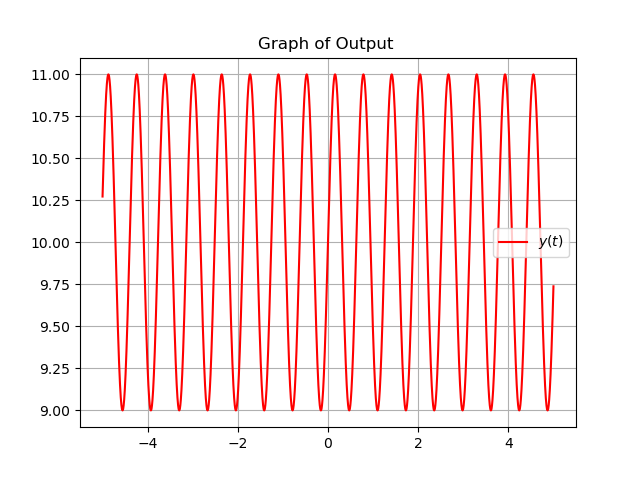
\includegraphics[width=\columnwidth]{2022/EE/37/figs/output.png}
    \caption{Output of the system, $y(t)$} 
\end{figure}
\begin{figure}[h]
    \centering
    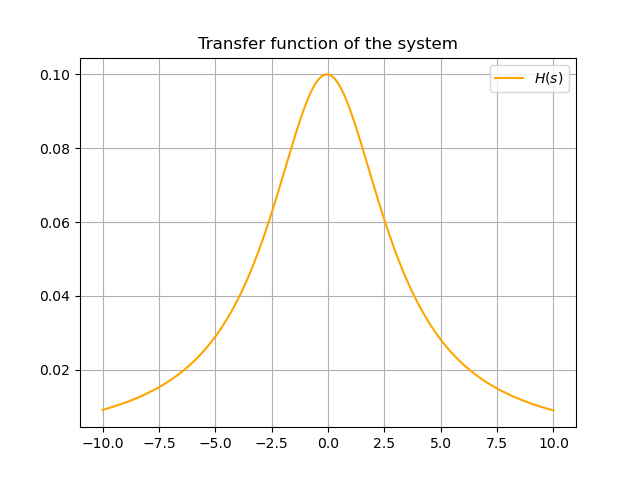
\includegraphics[width=\columnwidth]{2022/EE/37/figs/transfer.png}
    \caption{Transfer function of the system, $H(s)$} 
\end{figure}
% Properties of Laplace transform include 
% \begin{align}
%     ku\brak{t} &\system{L} \frac{k}{s}\label{37.Gate22.EE.eqn: 1}\\  
%     y\brak{t-k} & \system{L} e^{-sk} Y\brak{s} \label{37.Gate22.EE.eqn: 2}\\
%     \sin{\brak{\omega t}} &\system{L} \frac{\omega}{\omega^2 + s^2} \label{37.Gate22.EE.eqn: 3}
% \end{align}
% Taking Laplace transform of $x\brak{t}$, from \eqref{37.Gate22.EE.eqn: 1}, \eqref{37.Gate22.EE.eqn: 2} and \eqref{37.Gate22.EE.eqn: 3}
% \begin{align}
%     %a+b \sin{\brak{10t+\theta}} \system{L} 
%     1+0.1 \sin{\brak{10t}} &\system{L} \frac{1}{s} + 0.1 \frac{10}{s^2+10^2}\\
%  %   &\system{L} \frac{s^2+s+100}{s^2+100}\\
%     \implies X\brak{s} &= \frac{s^2+s+100}{s\brak{s^2+100}} \label{37.Gate22.EE.eqn: 5}
% \end{align}
% From \tabref{37.Gate22.EE.tab: 1},
% \begin{align}
%     G\brak{s}= \frac{Y\brak{s}}{X\brak{s}}=\frac{100}{s^2+0.1s+10} \\
%     \implies Y\brak{s}=X\brak{s} \brak{ \frac{100}{s^2+0.1s+10}}
% \end{align}
% From \eqref{37.Gate22.EE.eqn: 5}
% \begin{align}
%     Y\brak{s}= \frac{s^2+s+100}{s\brak{s^2+100}} \frac{100}{s^2+0.1s+10}\\
%     Y\brak{s}= 100 
% \end{align}
% Consider 
% \begin{align}
%     x(t) = x_1(t)+x_2(t)
% \end{align}
% where $x_1(t)=u(t)$ and $x_2(t)=0.1\sin{(10t)}u(t)$. 
% Since the given system is linear, 
% \begin{align}
%     y(t)=y_1(t)+y_2(t)
% \end{align}
% Where $y_1(t)$ and $y_2(t)$ are the outputs to $x_1(t)$ and $x_2(t)$ respectively.
% \begin{align}
%     y(t) \system{L} Y(s)\\
%     Y_1(s)=G(s)X_1(s)\\
%     Y_1(s)=\frac{1}{s}\brak{\frac{100}{s^2+0.1s+10}} 
% \end{align}
% By partial fractions 
% \begin{align}
%     Y_1(s)=
% \end{align}
% Consider 
% \begin{align}
%     G(s)&\system{L^{-0}}g(t)\\
%     G(s)&=\frac{100}{s^2+0.1s+10}\\
%     &=\frac{100}{(s^+0.05)^2 + 10 - (0.05)^2}\\
% \end{align}
% Let $\brak{10-\brak{0.05}^2}=a^2$ 
% \begin{align}
%     G(s)&=\frac{100}{a}\frac{a}{(s+0.05)^2+a^2}
% \end{align}
% From \eqref{37.Gate22.EE.eqn: 1}, \eqref{37.Gate22.EE.eqn: 2} and \eqref{37.Gate22.EE.eqn: 3}
% \begin{align}
%     g(t)=\frac{100}{a} e^{-0.05t}\sin{(at)}u(t)
% \end{align}
% The output of the system $y(t)$ is given by $$y(t)=x(t)*h(t)$$
% \begin{align}
%     y(t)=&\int_{-\infty}^{\infty} g(u)x(t-u) du\\
%     =&\int_{0}^{\infty} \frac{100}{a} e^{-0.05u}\sin{(au)}du \\&+ \int_{0}^{\infty} \frac{100}{a} e^{-0.05u}\sin{(au)}(0.1\sin{10(t-u)})\\
%     =&\brak{\frac{100}{a}\frac{e^{-0.05u}}{(-0.05)^2+a^2}\brak{(-0.05)\sin{au}-a\cos{au}}}_0^{\infty}\\
%     &+\int_{0}^{\infty} \frac{100}{a} e^{-0.05u}\sin{(au)}(0.1\sin{10(t-u)})\\
%     &=\frac{100}{a^2+(0.05)^2}+
% \end{align}
\end{enumerate}

 
